%
% ---------------------------------------------------------------
% Copyright (C) 2012-2018 Gang Li
% ---------------------------------------------------------------
%
% This work is the default powerdot-tuliplab style test file and may be
% distributed and/or modified under the conditions of the LaTeX Project Public
% License, either version 1.3 of this license or (at your option) any later
% version. The latest version of this license is in
% http://www.latex-project.org/lppl.txt and version 1.3 or later is part of all
% distributions of LaTeX version 2003/12/01 or later.
%
% This work has the LPPL maintenance status "maintained".
%
% This Current Maintainer of this work is Gang Li.
%
%latex slides.tex 
%dvips slides.dvi
%ps2pdf slides.ps
\documentclass[
 size=14pt,
 paper=smartboard,  %a4paper, smartboard, screen
 mode=present, 		%present, handout, print
 display=slides, 	% slidesnotes, notes, slides
 style=tuliplab,  	% TULIP Lab style
 pauseslide,
 fleqn,leqno]{powerdot}

\usepackage{cancel}
\usepackage{caption}
\usepackage{stackengine}
\usepackage{smartdiagram}
\usepackage{attrib}
\usepackage{amssymb}
\usepackage{amsmath} 
\usepackage{amsthm} 
\usepackage{mathtools}
\usepackage{rotating}
\usepackage{graphicx}
\usepackage{boxedminipage}
\usepackage{rotate}
\usepackage{calc}
\usepackage[absolute]{textpos}
\usepackage{psfrag,overpic}
\usepackage{fouriernc}
\usepackage{pstricks,pst-3d,pst-grad,pstricks-add,pst-text,pst-node,pst-tree}
\usepackage{moreverb,epsfig,subfigure}
\usepackage{color}
\usepackage{booktabs}
\usepackage{etex}
\usepackage{breqn}
\usepackage{multirow}
\usepackage{natbib}
\usepackage{bibentry}
\usepackage{gitinfo2}
\usepackage{siunitx}
\usepackage{nicefrac}
\usepackage{media9}
\usepackage{animate}
\usepackage{auto-pst-pdf}
\usepackage{breakurl}
\usepackage{fontawesome}
\usepackage{xcolor}
\usepackage{multicol}



\usepackage{verbatim}
\usepackage[utf8]{inputenc}
\usepackage{dtk-logos}
\usepackage{tikz}
\usepackage{adigraph}
\usepackage{hyperref}
\usepackage{pgfplots}
\usepackage{verbatim}
\usepackage{fontawesome}


\usepackage{todonotes}
\usepackage{animate}
\usepackage{fontawesome}

\usepackage{listings}
\lstset{frameround=fttt,
frame=trBL,
stringstyle=\ttfamily,
backgroundcolor=\color{yellow!20},
basicstyle=\footnotesize\ttfamily}
\lstnewenvironment{code}{
\lstset{frame=single,escapeinside=`',
backgroundcolor=\color{yellow!20},
basicstyle=\footnotesize\ttfamily}
}{}


\usepackage{hyperref}
\hypersetup{ % TODO: PDF meta Data
  pdftitle={Presentation Title},
  pdfauthor={Gang Li},
  pdfpagemode={FullScreen},
  pdfborder={0 0 0}
}


% \usepackage{auto-pst-pdf}
% package to show source code

\definecolor{LightGray}{rgb}{0.9,0.9,0.9}
\newlength{\pixel}\setlength\pixel{0.000714285714\slidewidth}
\setlength{\TPHorizModule}{\slidewidth}
\setlength{\TPVertModule}{\slideheight}
\newcommand\highlight[1]{\fbox{#1}}
\newcommand\icite[1]{{\footnotesize [#1]}}

\newcommand\twotonebox[2]{\fcolorbox{pdcolor2}{pdcolor2}
{#1\vphantom{#2}}\fcolorbox{pdcolor2}{white}{#2\vphantom{#1}}}
\newcommand\twotoneboxo[2]{\fcolorbox{pdcolor2}{pdcolor2}
{#1}\fcolorbox{pdcolor2}{white}{#2}}
\newcommand\vpspace[1]{\vphantom{\vspace{#1}}}
\newcommand\hpspace[1]{\hphantom{\hspace{#1}}}
\newcommand\COMMENT[1]{}

\newcommand\placepos[3]{\hbox to\z@{\kern#1
        \raisebox{-#2}[\z@][\z@]{#3}\hss}\ignorespaces}

\renewcommand{\baselinestretch}{1.2}


\newcommand{\draftnote}[3]{
	\todo[author=#2,color=#1!30,size=\footnotesize]{\textsf{#3}}	}
% TODO: add yourself here:
%
\newcommand{\gangli}[1]{\draftnote{blue}{GLi:}{#1}}
\newcommand{\shaoni}[1]{\draftnote{green}{sn:}{#1}}
\newcommand{\gliMarker}
	{\todo[author=GLi,size=\tiny,inline,color=blue!40]
	{Gang Li has worked up to here.}}
\newcommand{\snMarker}
	{\todo[author=Sn,size=\tiny,inline,color=green!40]
	{Shaoni has worked up to here.}}

%%%%%%%%%%%%%%%%%%%%%%%%%%%%%%%%%%%%%%%%%%%%%%%%%%%%%%%%%%%%%%%%%%%%%%%%
% title
% TODO: Customize to your Own Title, Name, Address
%
\title{Predict future sales}
\author{
Pengcheng Jiang
\\
\\JiLin University
}
\date{\gitCommitterDate}


% Customize the setting of slides
\pdsetup{
% TODO: Customize the left footer, and right footer
rf=\href{http://www.tulip.org.au}{
Last Changed by: \textsc{\gitCommitterName}\ \gitVtagn-\gitAbbrevHash\ (\gitAuthorDate)
},
cf={Predict future sales},
}


\begin{document}

\maketitle

\begin{slide}[toc=,bm=]{Overview}
\tableofcontents[content=currentsection,type=1]
\end{slide}

\section{Problem Definition}

%%==========================================================================================
%%
\begin{slide}[toc=,bm=]{Predict future sales}
  \begin{center}
  \begin{itemize}
  \item given: a challenging time-series dataset consisting of daily sales data, kindly provided by one of the largest Russian software firms - 1C Company.
  \item target: predict total sales for every product and store in the next month
  \item evaluation: Submissions are evaluated by root mean squared error (RMSE)
  \end{itemize}
  \end{center}
\end{slide}
%%
%%==========================================================================================

\section{Data Cleaning}
%%==========================================================================================
%%
\begin{slide}[toc=,bm=]{Date}
\begin{itemize}
  \item item_categories.csv:item_category_name	item_category_id\par
  \smallskip
  \item items.csv:item_id	item_category_id\par
  \item sales_train.csv:date  date_block_num  shop_id  item_id  item_price item_cnt_day\par
  \item shops.csv:shop_name	shop_id\par
  \item test.csv:shop_id  item_id\par
\end{itemize}
\end{slide}
%%
%%==========================================================================================


%%==========================================================================================
%%
\begin{slide}[toc=,bm=]{Data Information}
  sales_train:\par
    \begin{itemize}
      \item 2935849 rows,6 columns
      \item 21807 items,60 shops
      \item data_type
            \begin{itemize}
              \item data: object
              \item date_block_num: int
              \item shop_id:int
              \item item_id:int
              \item item_price:float
              \item item_cnt_day:float
            \end{itemize}
    \end{itemize}
\end{slide}
%%
%%==========================================================================================


%%==========================================================================================
%%
\begin{slide}[toc=,bm=]{Data Information}
  test:\par
    \begin{itemize}
      \item 214200 rows,3 columns
      \item 5100 items,40 shops
      \item data_type
            \begin{itemize}
              \item ID:int
              \item shop_id:int
              \item item_id:int
            \end{itemize}
    \end{itemize}
    From here you can see a lot of stores, goods in training set are not in the test set
\end{slide}
%%
%%==========================================================================================



%%==========================================================================================
%%
\begin{slide}[toc=,bm=]{Missing Value and Non Value}
  target:Find out whether there are empty values or missing values in the data\par
  result:\par
  missing value:0\par
  nan value:0\par
\end{slide}
%%
%%==========================================================================================


%%==========================================================================================
%%
\begin{slide}[toc=,bm=]{Data leakages}
  target:delete stores, goods in training set but not in the test set\par
  result:\par
  \setlength\parindent{2em}sales_train\par
  \setlength\parindent{4em}rows:1224439\par
    \setlength\parindent{4em}items:4716\par
    \setlength\parindent{4em}shops:42\par
\end{slide}
%%
%%==========================================================================================


%%==========================================================================================
%%
\begin{slide}[toc=,bm=]{Data duplication}
  target:See if duplicate items exist in the dataset\par
  result:\par
    \setlength\parindent{2em}sales_train:6\par
    \setlength\parindent{2em}test:0\par
  operation:delete duplications
\end{slide}
%%
%%==========================================================================================

%%==========================================================================================
%%
\begin{slide}[toc=,bm=]{Outliers}
  target:Calculate the outliers of item_cnt_day and item price\par
  result:
\end{slide}
%%
%%==========================================================================================

%%==========================================================================================
%%
\begin{slide}[toc=,bm=]{Outliers}
  \begin{figure}
    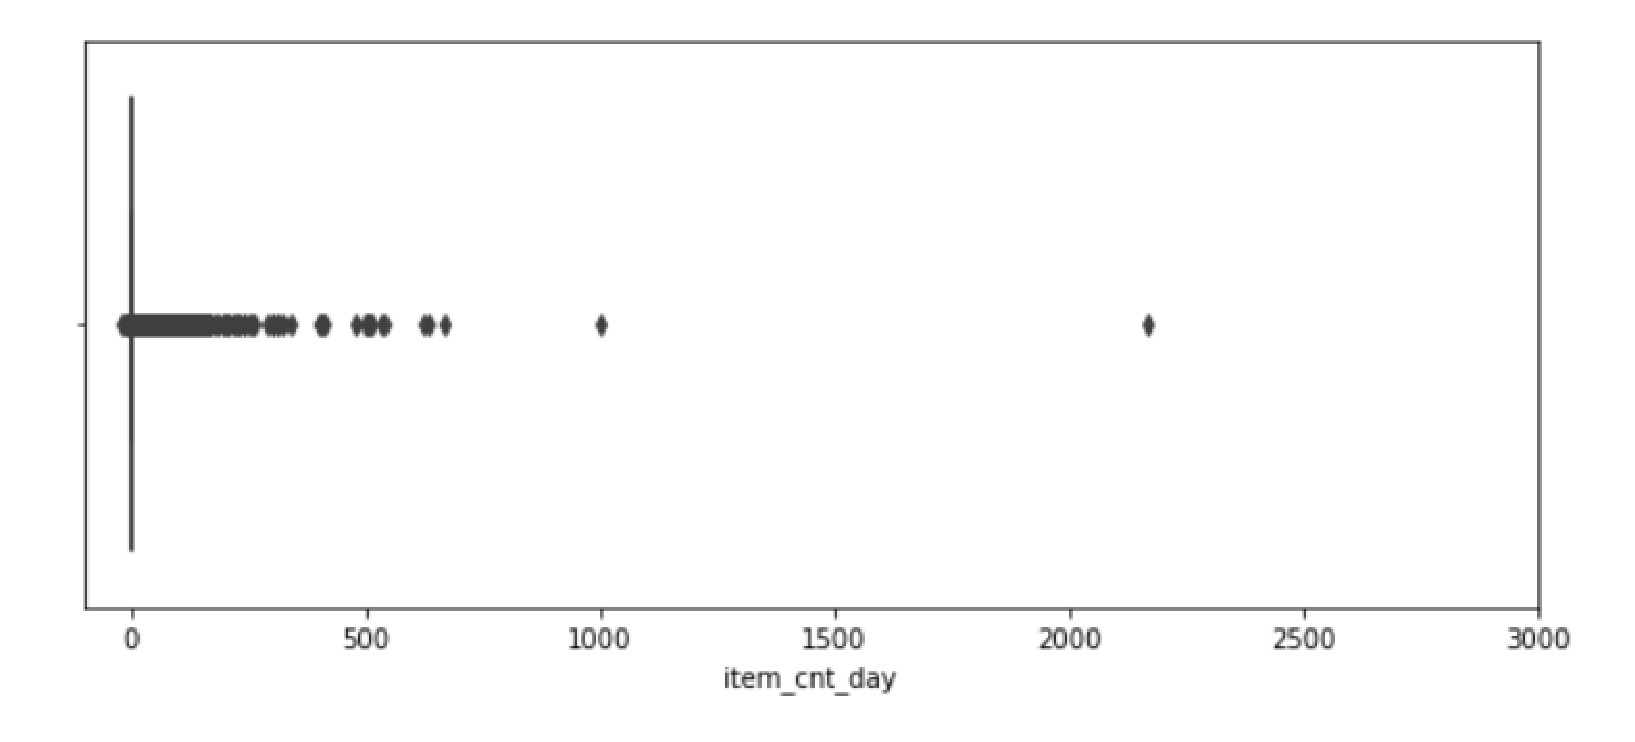
\includegraphics[scale=0.5]{picture/data_7.eps}
  \end{figure}
\end{slide}
%%
%%==========================================================================================

%%==========================================================================================
%%
\begin{slide}[toc=,bm=]{Outliers}
  \begin{figure}
    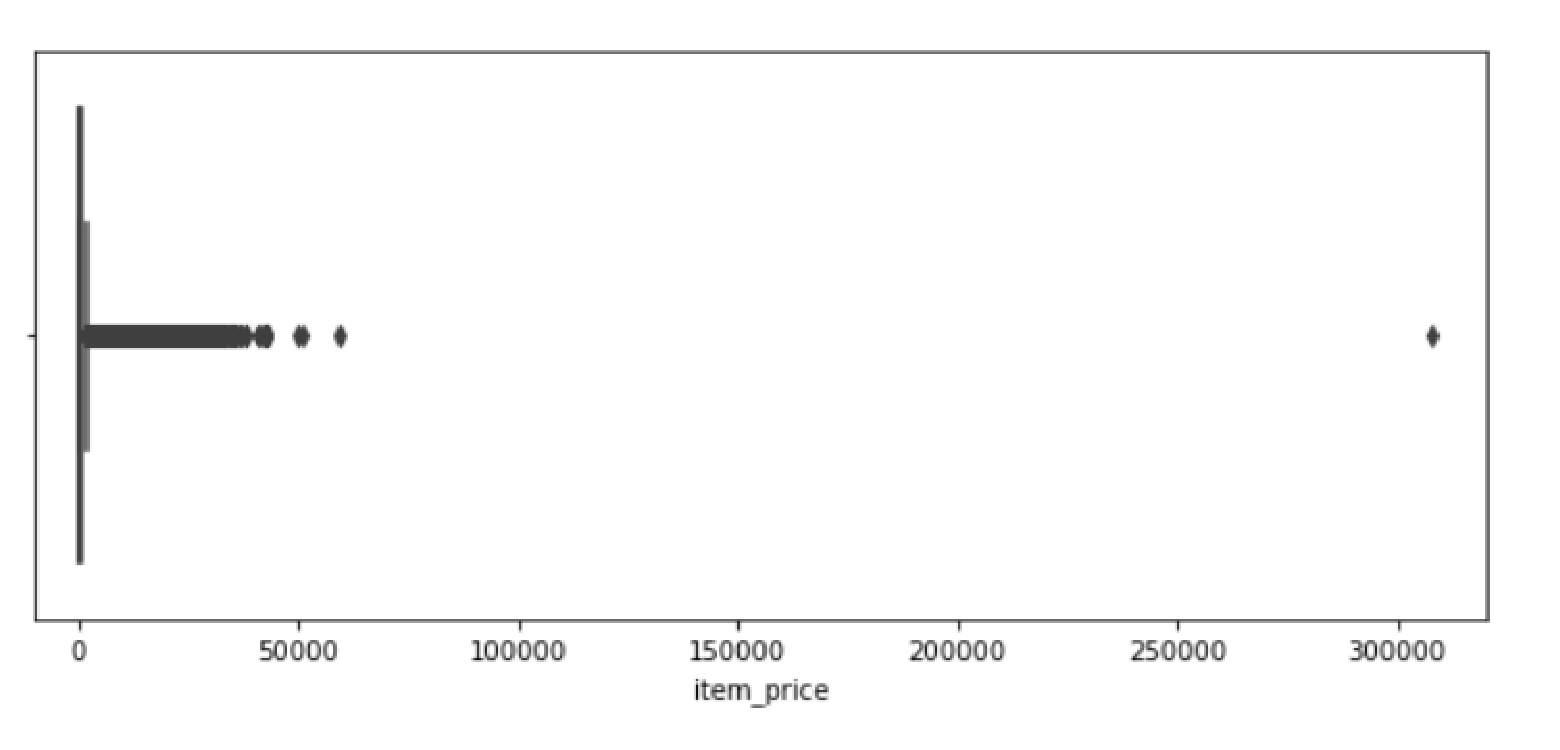
\includegraphics[scale=0.5]{picture/data_8.eps}
  \end{figure}
\end{slide}
%%
%%==========================================================================================

%%==========================================================================================
%%
\begin{slide}[toc=,bm=]{outdated items}
  target:Analyze how many products have not been sold in the last six consecutive months. How many of these products appear in the test set.
  result:
  There are 12391 training sets, which have not been sold in the last six months.
  There are 164 test sets, which have not been sold in the last six months
\end{slide}
%%
%%==

%%==========================================================================================
%%
\begin{slide}[toc=,bm=]{Negative}
  Change item whose commodity price is negative to median
  operation:
\end{slide}
%%
%%==========================================================================================


\section{Data analysis}

%%==========================================================================================
%%
\begin{slide}[toc=,bm=]{Monthly sales of goods}
  \begin{figure}
    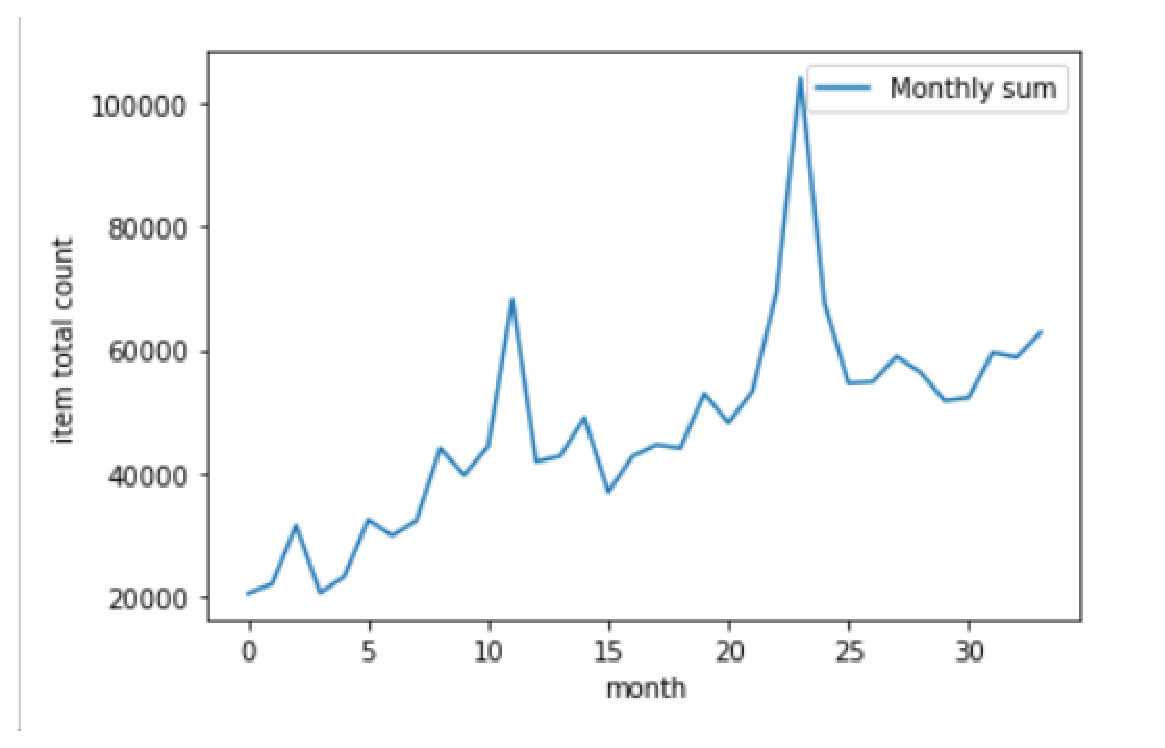
\includegraphics[scale=0.5]{picture/data_20.eps}
  \end{figure}
    Explain that the month is related to the sales volume of goods: the sales volume at the end of the year is increasing
\end{slide}
%%
%%==========================================================================================


%%==========================================================================================
%%
\begin{slide}[toc=,bm=]{Shop sales}
  \begin{figure}
    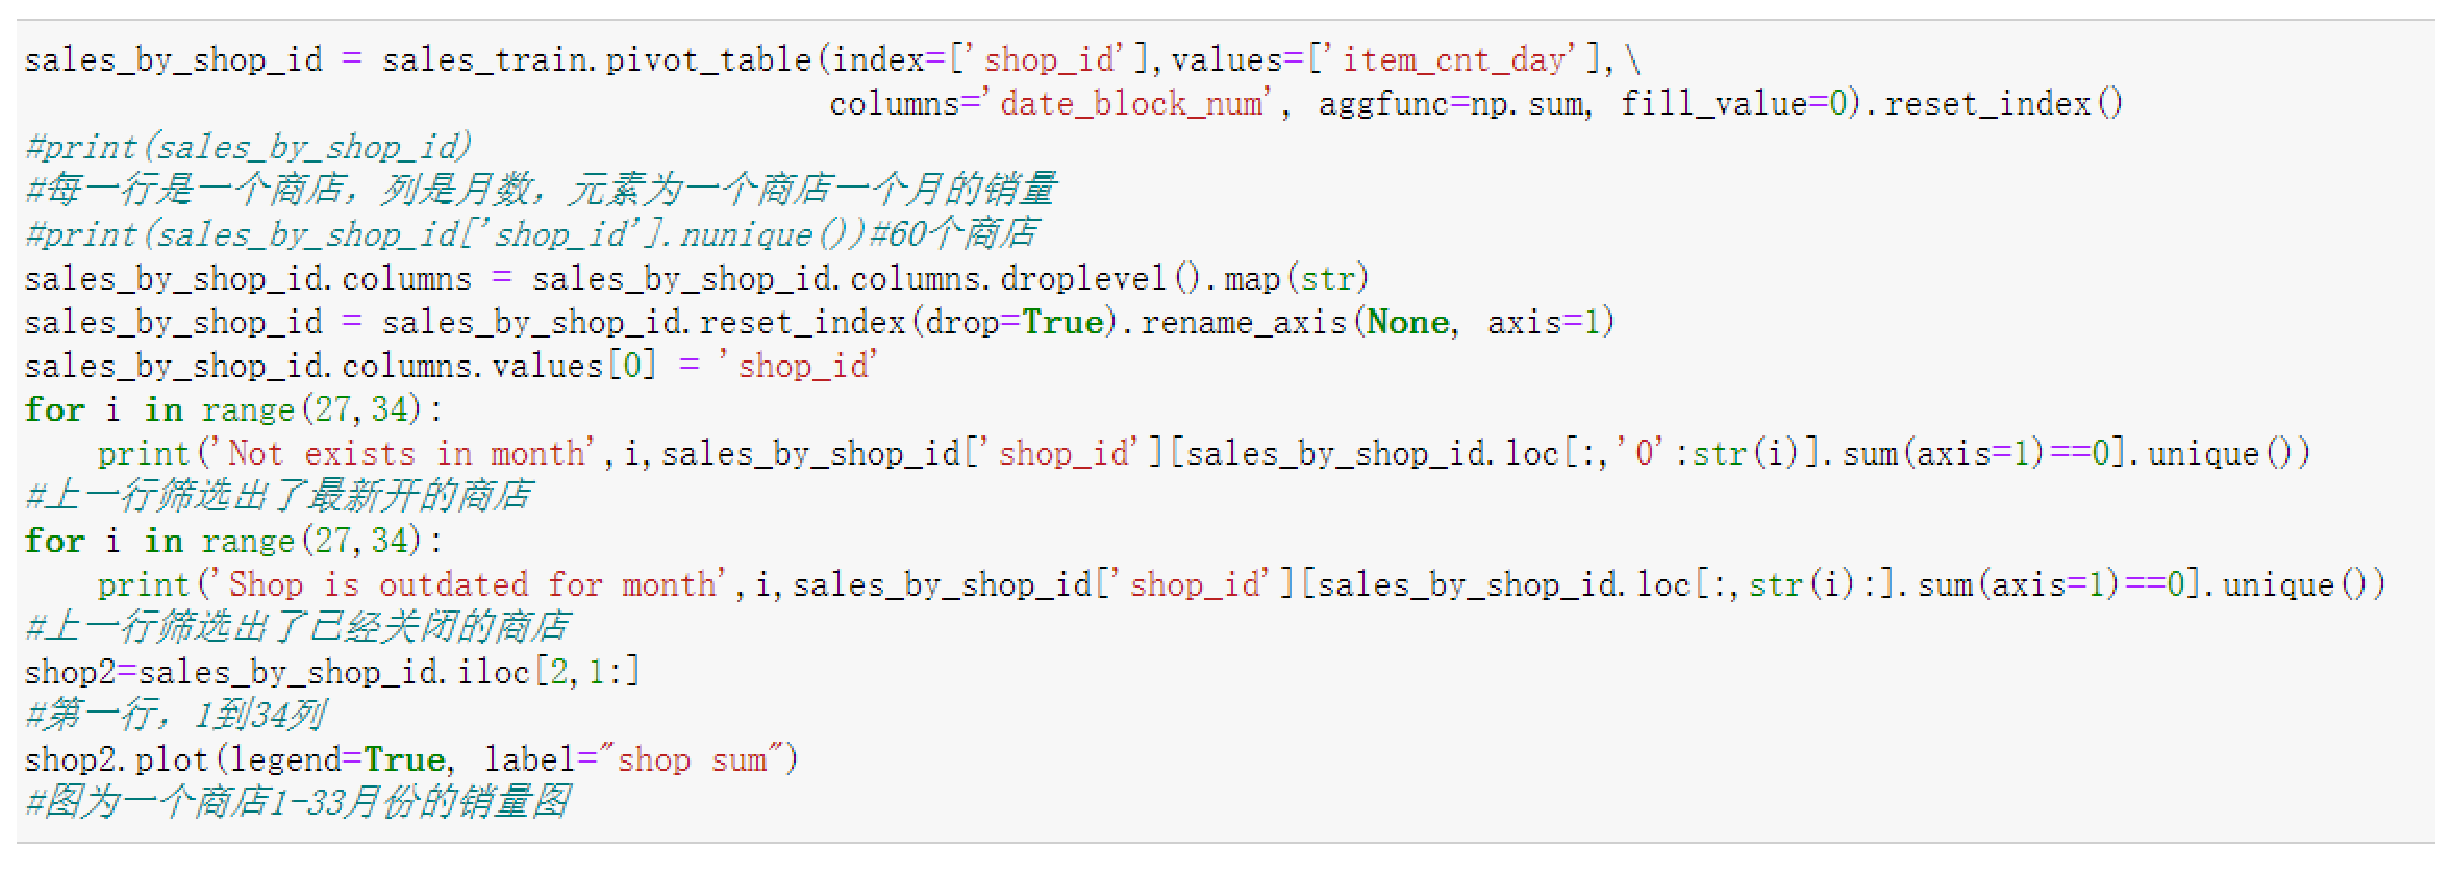
\includegraphics[scale=0.5]{picture/data_10.eps}
  \end{figure}
  \begin{center}
    Objective: To prepare for feature extraction
  \end{center}
\end{slide}
%%
%%==========================================================================================


%%==========================================================================================
%%
\begin{slide}[toc=,bm=]{Shop sales}
  \begin{figure}
    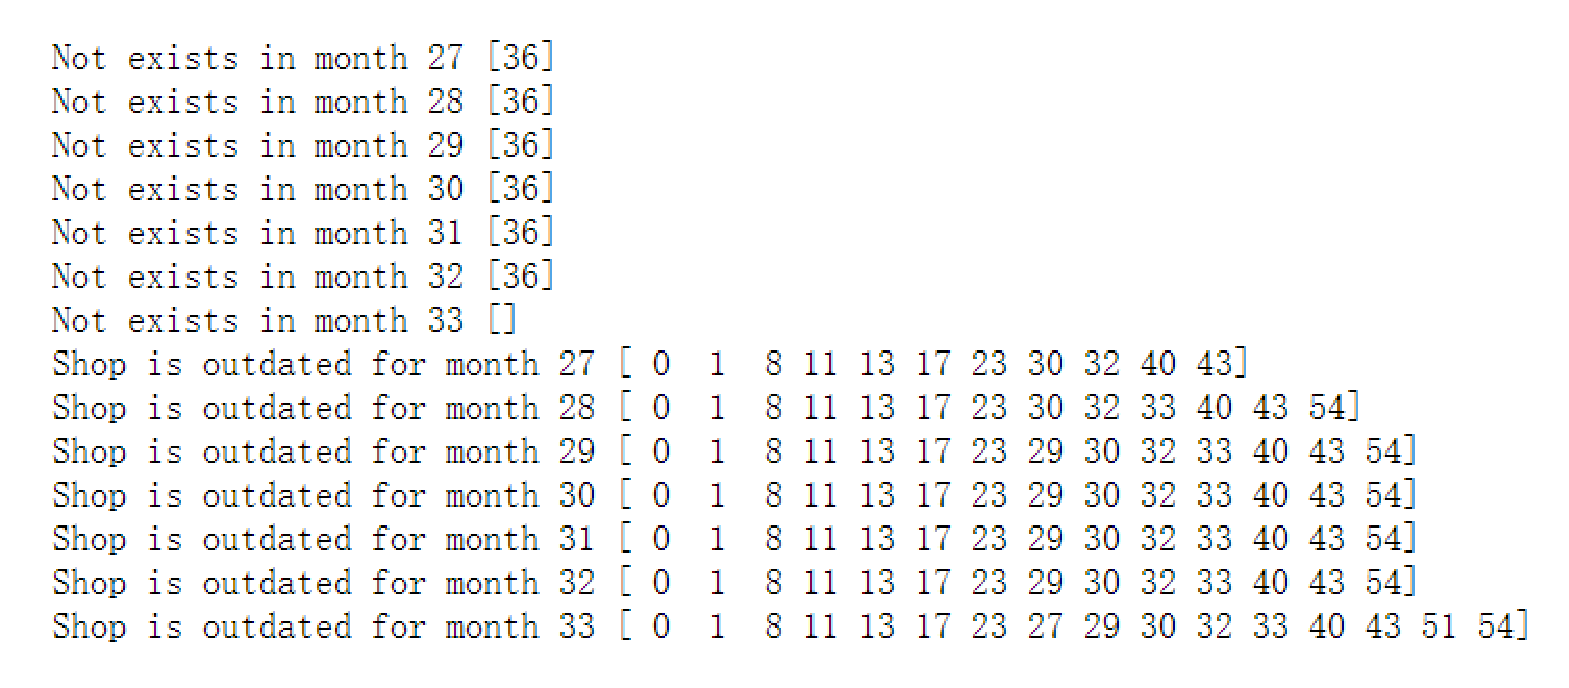
\includegraphics[scale=0.5]{picture/data_11.eps}
  \end{figure}
\end{slide}
%%
%%==========================================================================================

%%==========================================================================================
%%
\begin{slide}[toc=,bm=]{Item Information}
  The categories of items are: large categories, small categories, we separate them, and code them separately to facilitate subsequent feature extraction
  \begin{figure}
    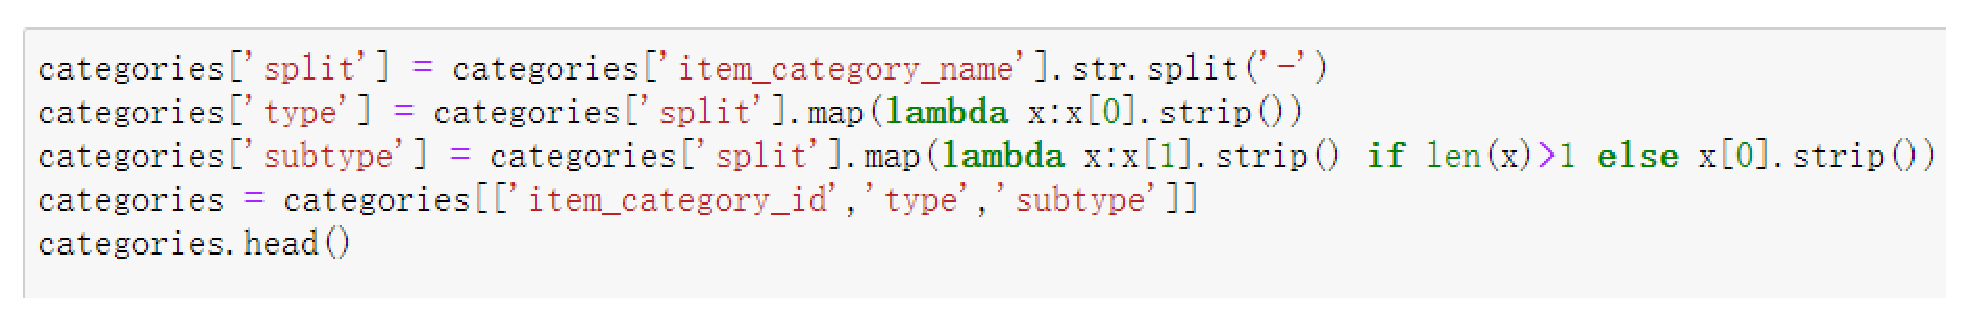
\includegraphics[scale=0.5]{picture/data_13.eps}
  \end{figure}
\end{slide}
%%
%%==========================================================================================



%%==========================================================================================
%%
\begin{slide}[toc=,bm=]{Shop Information}
  Shop information includes: the city where the store is located, the type of store, which we separate and encode separately for subsequent feature extraction
\end{slide}
%%
%%==========================================================================================





%%==========================================================================================
%%
\begin{slide}[toc=,bm=]{Shop Information}
  \begin{figure}
    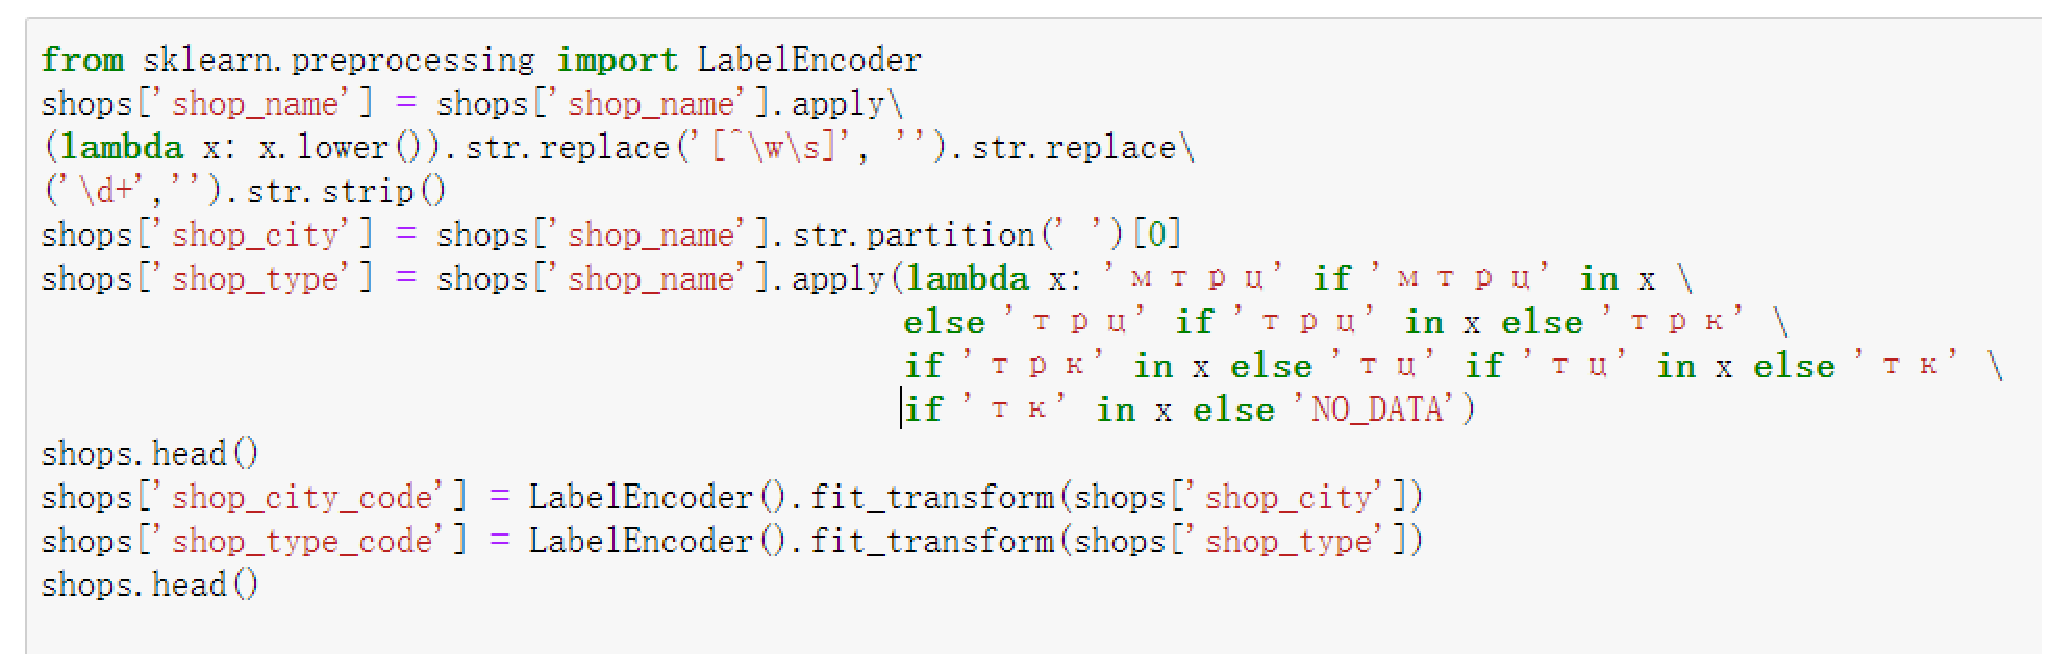
\includegraphics[scale=0.5]{picture/data_12.eps}
  \end{figure}
\end{slide}
%%
%%==========================================================================================


%%==========================================================================================
%%
\begin{slide}[toc=,bm=]{Items Information}
  The training set contains only the items that the store actually sold that month,
  for items not sold during the month, you should add them and set them to 0
  \begin{figure}
    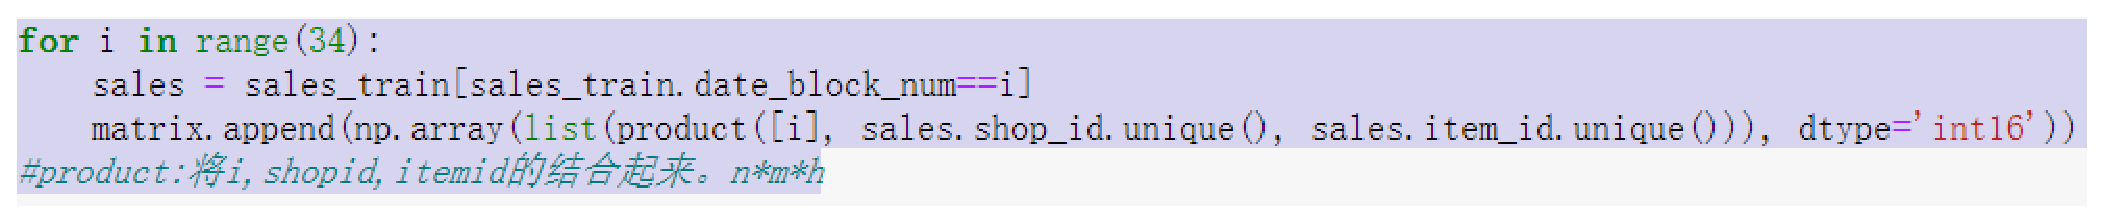
\includegraphics[scale=0.5]{picture/data_15.eps}
  \end{figure}
   Cartesian product
\end{slide}
%%
%%==========================================================================================

%%==========================================================================================
%%
\begin{slide}[toc=,bm=]{Monthly total sales}
 
  \begin{figure}
    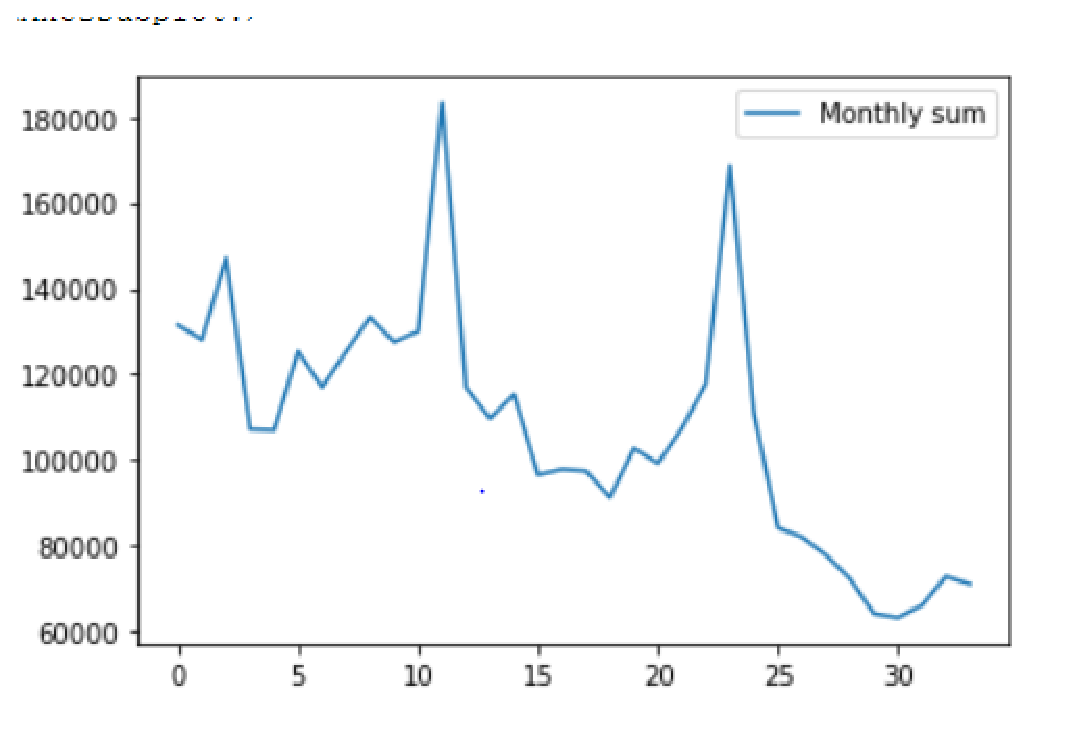
\includegraphics[scale=0.5]{picture/data_18.eps}
  \end{figure}
\end{slide}
%%
%%==========================================================================================

%%==========================================================================================
%%
\begin{slide}[toc=,bm=]{Sales per store}
  It is known that the city to which the store belongs and the type of store affect sales
  \begin{figure}
    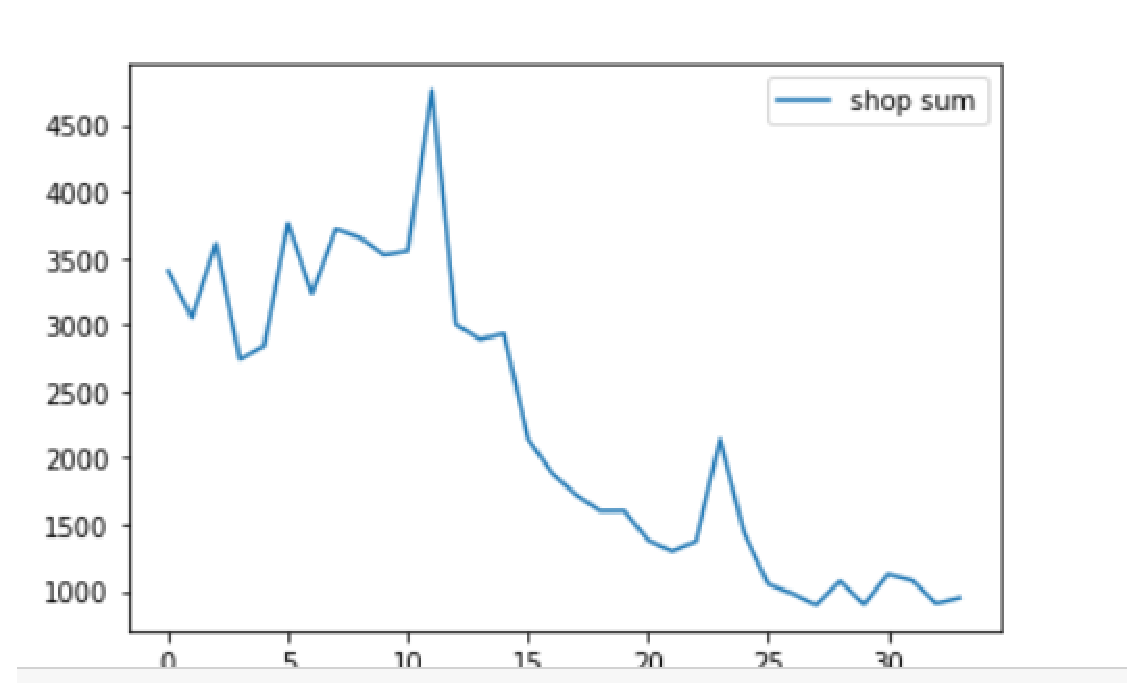
\includegraphics[scale=0.5]{picture/data_19.eps}
  \end{figure}
\end{slide}
%%
%%==========================================================================================


\section{Model}


%%==========================================================================================
%%
\begin{slide}[toc=,bm=]{Model selection}
  \begin{itemize}
    \item GBDT
    \item Xgboost
    \item lightgbm
    \item neural network
  \end{itemize}
\end{slide}
%%
%%==========================================================================================


%%==========================================================================================
%%
\begin{slide}[toc=,bm=]{Method One}
  Method:The sales of the 34th month are regarded as the sales of the 35th month\par
  operation:Count the sales volume of each item in each store in the 33rd month and merge it with test
  Result:RMSE=1.16777
\end{slide}
%%
%%==========================================================================================


%%==========================================================================================
%%
\begin{slide}[toc=,bm=]{Method One}
  features:shop_id,item_id,item_cnt_month\par
  Method:lightgbm
  \begin{figure}
    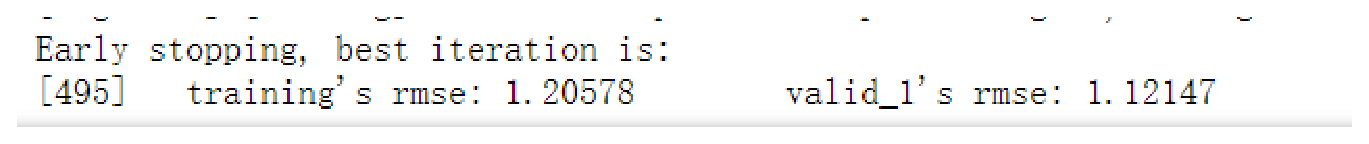
\includegraphics[scale=0.5]{picture/data_14.eps}
  \end{figure}
  attention:After some data preprocessing
\end{slide}
%%
%%==========================================================================================

%%==========================================================================================
%%
\begin{slide}[toc=,bm=]{Method Two}
  Some historical information needs to be generated by delayed operations. For example, you can use the 0-33 month sales as a historical feature of the 1-34 month (one month delay).
\end{slide}
%%
%%==========================================================================================

%%==========================================================================================
%%
\begin{slide}[toc=,bm=]{Method Two}
  \begin{itemize}
    \item Historical information on monthly sales (per item-store).
    \item Historical information on the average monthly sales (all merchandise-store) value
    \item Average monthly sales (per item) and historical characteristics
    \item Average monthly sales (per store) and historical characteristics
    \item Average monthly sales (per commodity category) and historical characteristics
    \item Average monthly sales (commodity category-store) and historical characteristics
    \item Average and historical characteristics of monthly sales volume (commodity category _ class)
    \item Average and historical characteristics of monthly sales (commodity-commodity category _ class)
    \item Average monthly sales (store _ city) and historical characteristics
    \item Average monthly sales (merchandise-store-city) and historical characteristics
    \item Trends, price changes over the past six months
    \item Number of days per month
    \item Sales beginning and ending
  \end{itemize}
\end{slide}
%%
%%==========================================================================================

%%==========================================================================================
%%
\begin{slide}[toc=,bm=]{Method Two}
  \begin{figure}
    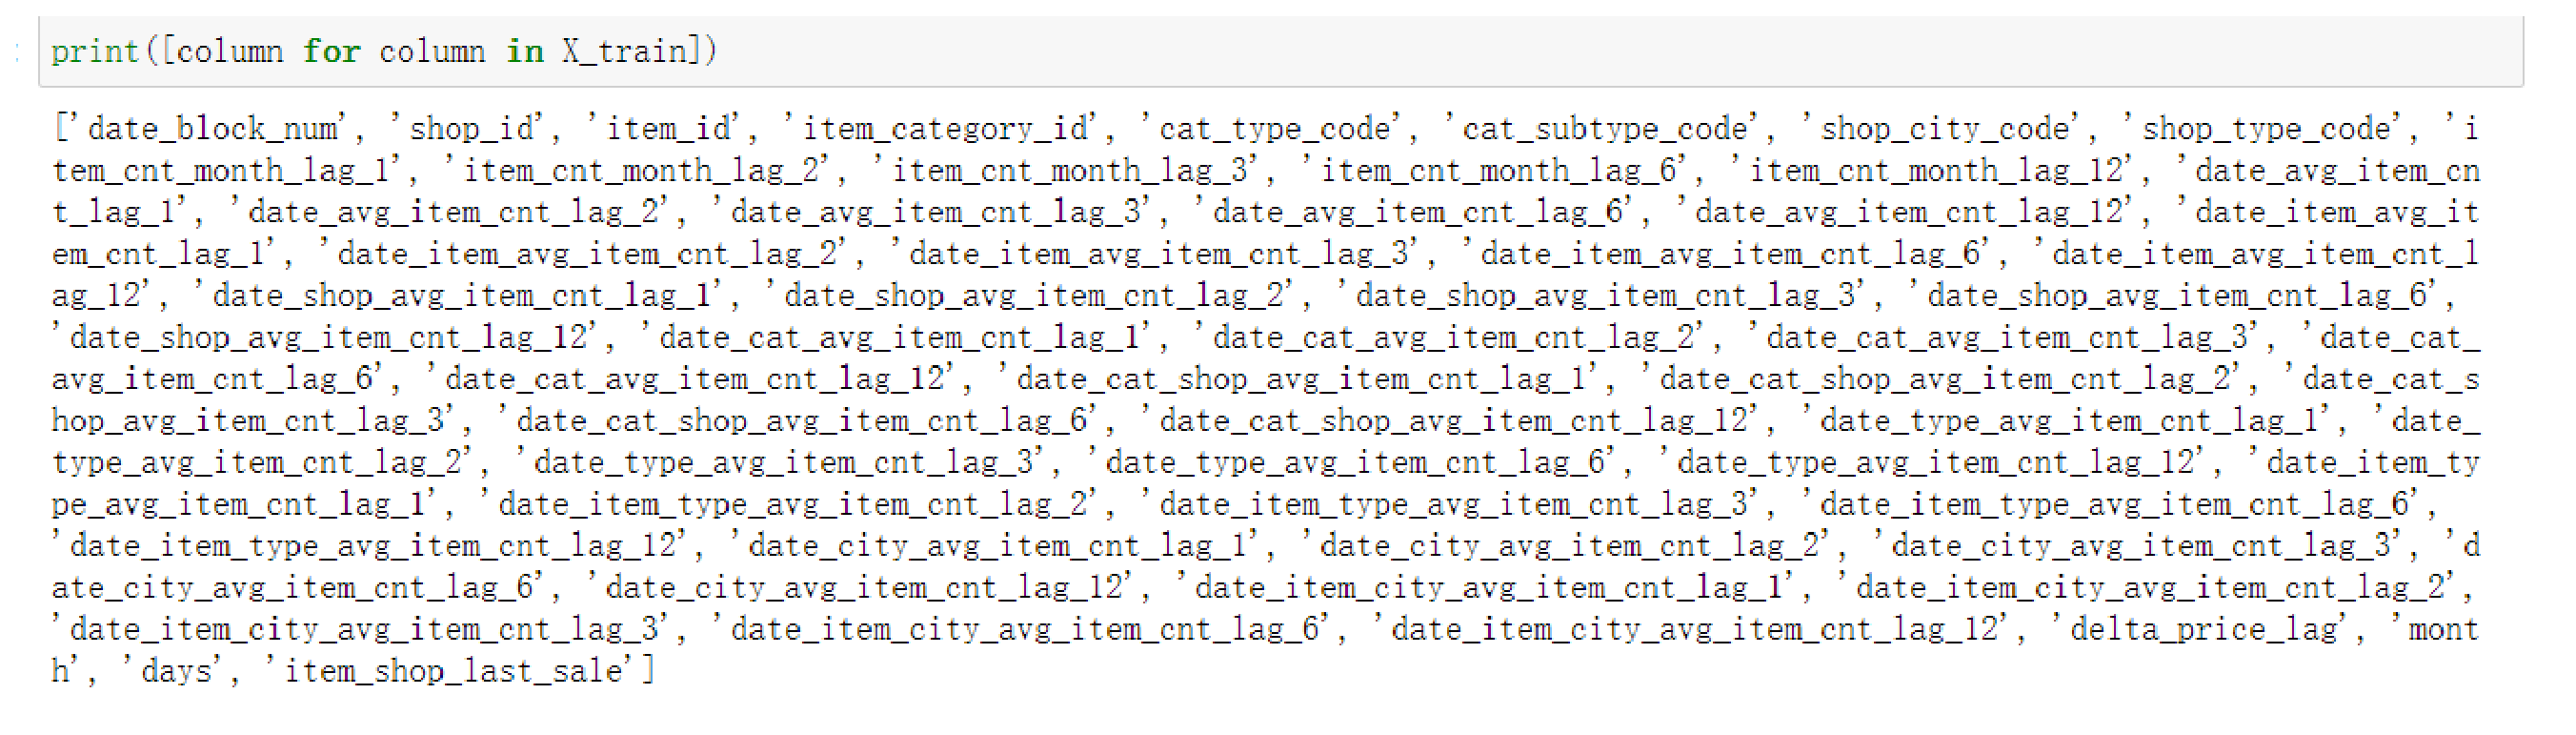
\includegraphics[scale=0.5]{picture/data_16.eps}
  \end{figure}
\end{slide}
%%
%%==========================================================================================

%%==========================================================================================
%%
\begin{slide}[toc=,bm=]{Method Two}
  \begin{figure}
    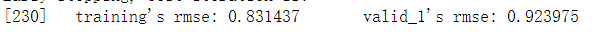
\includegraphics[scale=0.5]{picture/data_17.eps}
  \end{figure}
\end{slide}
%%
%%==========================================================================================

\section{Lightgbm}

\end{document}
